\documentclass[border=0.25cm]{standalone}
\usepackage{xcolor}
\usepackage{tikz}
\usetikzlibrary{arrows, arrows.meta}
\tikzset{    
    barbarrow/.style={ % style that just defines the arrow tip
        >={Straight Barb[left,length=5pt,width=5pt]},
        thick,
        <->
    },
    blues/.style={
        color=blue
    },
    reds/.style={
        color=red
    }
}
\definecolor{light-gray}{gray}{0.975}
\definecolor{pcolor}{rgb}{0.21, 0.27, 0.31}
\begin{document}
\begin{tabular}{c c c c c}
\begin{tikzpicture}
    \tikzstyle{node1}=[draw,scale=0.01,shape=circle,color=red,fill=red] %
    \draw[color=light-gray, style=dashed] (0,0) grid (8,8);
    \node[above, scale=1.25] at (4,8) {Set of polygons A};
    \node[node1] (A) at (0,2) {}; %[node1]
    \node[node1] (C) at (2,0) {};
    \node[node1] (E) at (2,4) {};
    \node[node1] (K) at (4,2) {};
    \node[node1] (M) at (4,6) {};
    \node[node1] (R) at (6,4) {};
    \node[scale=1.5] at (0.5,3.5) {A};
    
    \draw[reds]
        (A) -- (C) (A) -- (E) (C) -- (K) (E) -- (K) 
        (E) -- (M) (K) -- (R) (M) -- (R);
\end{tikzpicture} 
&
\begin{tikzpicture}
    \draw[color=white, style=dashed] (0,0) grid (0,8);
    \node[scale=4] at (0, 4) {$\Longrightarrow$};
\end{tikzpicture} 
&
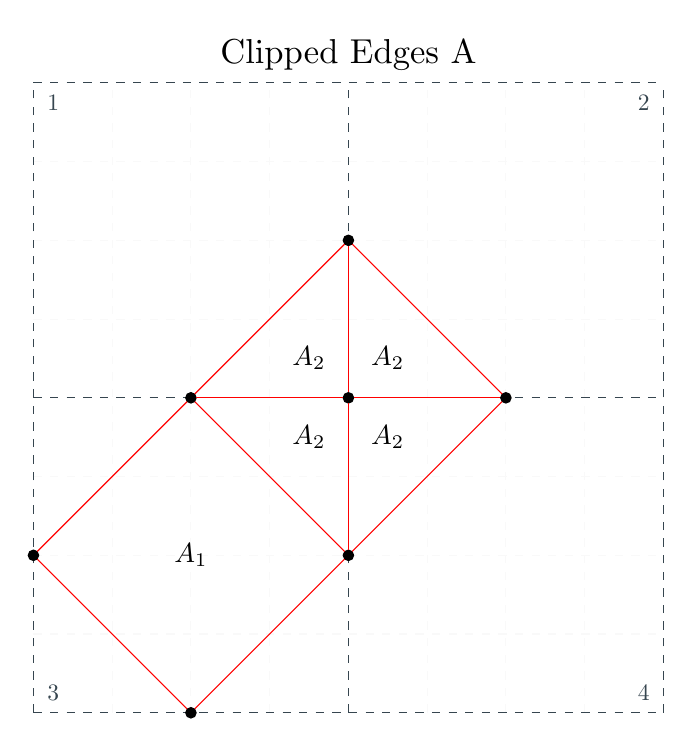
\begin{tikzpicture}
    \tikzstyle{node1}=[draw,scale=0.4,shape=circle,color=black,fill=black]
    \tikzstyle{node2}=[draw,scale=0.4,shape=circle,color=red,fill=red]
    \tikzstyle{text}=[draw,scale=0.5,color=black]
    \draw[color=light-gray, style=dashed] (0,0) grid (8,8);
    \draw[color=pcolor, style=dashed, step=4] (0,0) grid (8,8);
    \node[scale=0.85, color = pcolor] at (0.25, 7.75) {$1$};
    \node[scale=0.85, color = pcolor] at (7.75, 7.75) {$2$};
    \node[scale=0.85, color = pcolor] at (0.25, 0.25) {$3$};
    \node[scale=0.85, color = pcolor] at (7.75, 0.25) {$4$};
    
    \node[above, scale=1.25, thick] at (4,8) {Clipped Edges A};
    \node[node1] (A) at (0,2) {};
    \node[node1] (C) at (2,0) {};
    \node[node1] (E) at (2,4) {};
    \node[node1] (K) at (4,2) {};
    \node[node1] (M) at (4,6) {};
    \node[node1] (R) at (6,4) {};
    \node[node1] (Z) at (4,4) {};
    \node at (2,2) {$A_1$};
    \node at (3.5,4.5) {$A_2$};
    \node at (4.5,4.5) {$A_2$};
    \node at (3.5,3.5) {$A_2$};
    \node at (4.5,3.5) {$A_2$};
    
    \draw[reds](A) -- (C);\draw[reds](A) -- (E); 
    \draw[reds](C) -- (K);\draw[reds](E) -- (K); 
    \draw[reds](E) -- (M);\draw[reds](K) -- (R); 
    \draw[reds](M) -- (R);
    \draw[reds] (Z) -- (E);
    \draw[reds] (Z) -- (R);
    \draw[reds] (Z) -- (M);
    \draw[reds] (Z) -- (K);
\end{tikzpicture}
&
\begin{tikzpicture}
    \draw[color=white, style=dashed] (0,0) grid (0,8);
    \node[scale=4] at (0, 4) {$\Longrightarrow$};
\end{tikzpicture} 
&
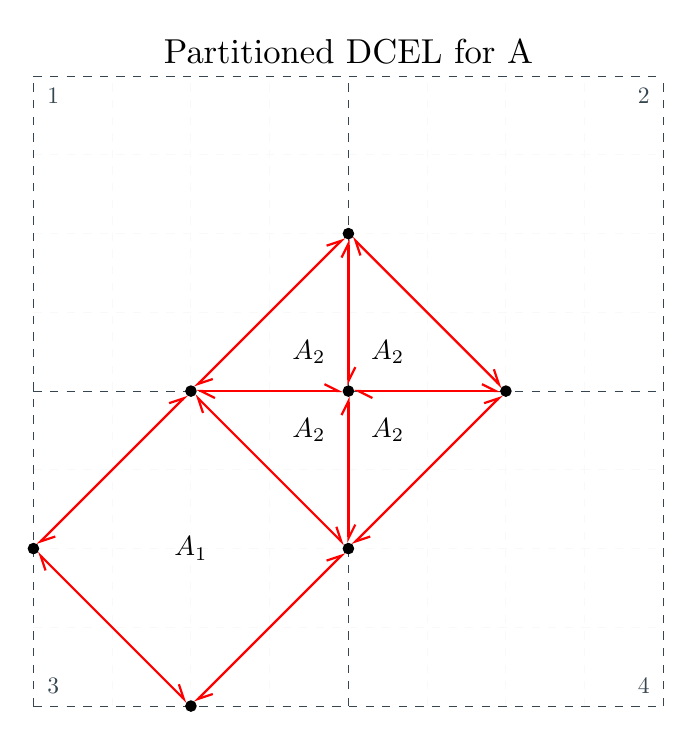
\begin{tikzpicture}
    \tikzstyle{node1}=[draw,scale=0.4,shape=circle,color=black,fill=black]
    \tikzstyle{node2}=[draw,scale=0.4,shape=circle,color=red,fill=red]
    \tikzstyle{text}=[draw,scale=0.5,color=black]
    \draw[color=light-gray, style=dashed] (0,0) grid (8,8);
    \draw[color=pcolor, style=dashed, step=4] (0,0) grid (8,8);
    \node[scale=0.85, color = pcolor] at (0.25, 7.75) {$1$};
    \node[scale=0.85, color = pcolor] at (7.75, 7.75) {$2$};
    \node[scale=0.85, color = pcolor] at (0.25, 0.25) {$3$};
    \node[scale=0.85, color = pcolor] at (7.75, 0.25) {$4$};

    \node[above, scale=1.25, thick] at (4,8) {Partitioned DCEL for A};
    \node[node1] (A) at (0,2) {};
    \node[node1] (C) at (2,0) {};
    \node[node1] (E) at (2,4) {};
    \node[node1] (K) at (4,2) {};
    \node[node1] (M) at (4,6) {};
    \node[node1] (R) at (6,4) {};
    \node[node1] (Z) at (4,4) {};
    \node at (2,2) {$A_1$};
    \node at (3.5,4.5) {$A_2$};
    \node at (4.5,4.5) {$A_2$};
    \node at (3.5,3.5) {$A_2$};
    \node at (4.5,3.5) {$A_2$};
    
    \draw[barbarrow, color=red] (A) -- (C); \draw[barbarrow, color=red] (A) -- (E); 
    \draw[barbarrow, color=red] (C) -- (K); \draw[barbarrow, color=red] (E) -- (K); 
    \draw[barbarrow, color=red] (E) -- (M); \draw[barbarrow, color=red] (K) -- (R); 
    \draw[barbarrow, color=red] (M) -- (R);
    \draw[barbarrow, color=red] (Z) -- (E);
    \draw[barbarrow, color=red] (Z) -- (R);
    \draw[barbarrow, color=red] (Z) -- (M);
    \draw[barbarrow, color=red] (Z) -- (K);
\end{tikzpicture}
\\
\end{tabular}
\end{document}
